% ============================================================
% SDN Testbed Paper — IEEE ICC 2027
% Reframed: open-source plug-and-play SDN benchmarking testbed
% ============================================================
\documentclass[conference]{IEEEtran}
\IEEEoverridecommandlockouts

% ── Packages ─────────────────────────────────────────────────
\usepackage{cite}
\usepackage{amsmath,amssymb,amsfonts}
\usepackage{algorithmic}
\usepackage{graphicx}
\usepackage{textcomp}
\usepackage{xcolor}
\usepackage{booktabs}
\usepackage{url}
% hyperref omitted: PDF link annotations not permitted by submission system.
\newcommand{\href}[2]{#2}
\providecommand{\hyperref}[2][]{#2}
\usepackage{makecell}
\usepackage{tikz}
\usetikzlibrary{shapes.geometric, arrows.meta, positioning, fit, calc}
\usepackage{subfigure}

% Symbols for comparison table
\usepackage{pifont}
\newcommand{\cmark}{\ding{51}}
\newcommand{\xmark}{\ding{55}}

% Reduce caption spacing
\setlength{\abovecaptionskip}{2pt}

% Reduce float spacing
\setlength{\textfloatsep}{8pt}
\setlength{\floatsep}{6pt}
\setlength{\intextsep}{6pt}

% ── Title ─────────────────────────────────────────────────────
\title{An Open-Source Plug-and-Play Testbed for Reproducible\\
SDN Controller Performance Benchmarking}

\author{
    \IEEEauthorblockN{Tamerlan Abdullayev}
    \IEEEauthorblockA{\textit{Department of Computer Science}\\
        University of Cincinnati\\
        Cincinnati, OH, USA\\
        abdulltn@mail.uc.edu}
    \and
    \IEEEauthorblockN{Giovani Abuaitah}
    \IEEEauthorblockA{\textit{Department of Computer Science}\\
        University of Cincinnati\\
        Cincinnati, OH, USA\\
        abuaitgi@ucmail.uc.edu}
}

\setlength{\columnsep}{0.13in}

\begin{document}

\maketitle

% ── Abstract ─────────────────────────────────────────────────
\begin{abstract}
Reproducible and rigorous benchmarking of Software-Defined Networking
(SDN) controllers remains an open challenge. Existing tools either
rely on synthetic traffic that fails to capture realistic
controller behavior, or consist of ad-hoc manual experiments that
lack statistical validation and can be challenging to reuse across studies.
We present an open-source, plug-and-play SDN benchmarking testbed
that combines Mininet, iperf3, and an instrumented Ryu controller
application into a fully automated, seed-controlled experimentation
pipeline. The testbed supports configurable topologies and
parameters, records per-event controller processing latency
(Packet-In to FlowMod dispatch), and produces statistically
validated results through repeated trials with inline aggregation.
To demonstrate the testbed, we execute 400 controlled experiments
across two topologies (star and fat-tree), five host counts,
and four flow rates with 10 repetitions per configuration.
The demonstration confirms that the testbed successfully captures
topology-dependent controller behavior and uncovers performance
differences that are invisible to existing benchmarking approaches. The testbed and all experiment
scripts are publicly available at:
\url{https://github.com/PLACEHOLDER/sdn-testbed}.
\end{abstract}

\begin{IEEEkeywords}
SDN, benchmarking, testbed, reproducibility, Mininet, OpenFlow,
controller performance, iperf3, open-source.
\end{IEEEkeywords}

% ── I. Introduction ──────────────────────────────────────────
\section{Introduction}
\label{sec:intro}

Software-defined networking (SDN)~\cite{McKeown2008OpenFlow}
decouples the control plane from the data plane, placing forwarding
intelligence in a software controller. The OpenFlow
protocol~\cite{McKeown2008OpenFlow} provides the standardized
southbound interface between controllers and switches, enabling
programmatic network control. As SDN deployments
scale~\cite{Kreutz2015SDNSurvey}, the ability to rigorously and
reproducibly benchmark controller performance becomes increasingly
important for research, controller selection, and capacity planning.

\textbf{The Reproducibility Gap.}
Despite the availability of several benchmarking tools, the SDN
research community lacks an open-source, end-to-end testbed that is
both statistically rigorous and reusable across studies.
Synthetic tools such as CBench~\cite{cbench2012},
OFLOPS~\cite{Rotsos2012OFLOPS}, and
WCBench~\cite{wcbench2015} inject artificial Packet-In bursts
to measure controller throughput but generate no real TCP flows,
perform no MAC learning, and may not capture the topology-driven
event dynamics that characterize realistic deployments.
The IETF's RFC~8456~\cite{rfc8456} defines a methodology for
SDN controller benchmarking---recommending varying topologies,
varying network sizes, and repeated statistical trials---yet
to the best of our knowledge, open-source implementations of
that methodology remain limited.

Recent academic studies that do use realistic emulation tools
such as Mininet and iPerf~\cite{Koulouras2022RealWorld,
Cabarkapa2022TreeTopology, Ali2024Comparison} rely on single,
manually executed runs between one host pair with no statistical
repetitions, no automated parameter sweeps, and no controller
instrumentation beyond end-to-end RTT. As a result, their
findings can be challenging to verify, extend, or reuse without
reconstructing the experimental setup independently.

\textbf{Our Contribution.}
We present an open-source, plug-and-play SDN benchmarking
testbed that addresses these gaps. The testbed makes the following
contributions:

\begin{itemize}
  \item \textbf{Automated, reproducible pipeline.} A seed-controlled,
  fully automated shell and Python pipeline orchestrates controller
  startup, network emulation, traffic generation, per-run
  aggregation, and cleanup. Any experiment can be exactly replicated
  from its seed without manual intervention.

  \item \textbf{Per-event controller instrumentation.} The testbed
  instruments the Ryu controller~\cite{RyuFramework} at the
  event level, recording wall-clock timestamps from Packet-In
  receipt to FlowMod dispatch for every control-plane event.
  This enables separation of median (p50) and tail (p95) latency,
  a distinction invisible to RTT-based measurements used in
  prior work.

  \item \textbf{Realistic concurrent traffic.} Traffic is generated
  by iperf3~\cite{iperf3} with concurrent, overlapping TCP flows
  between randomly selected host pairs, creating realistic
  simultaneous Packet-In events that stress the controller in
  ways that synthetic single-flow tests may not.

  \item \textbf{Plug-and-play extensibility.} Topologies and
  traffic parameters are configurable via command-line arguments.
  New topologies are added by implementing a single Python class.
  The architecture is designed for straightforward substitution
  of alternative controllers.

  \item \textbf{Statistical validation.} The pipeline supports
  configurable repetitions per configuration with distinct seeds,
  enabling standard deviation computation and confidence evaluation
  across trials.
\end{itemize}

To the best of our knowledge, this is among the first open-source
frameworks that aligns with the IETF RFC~8456 benchmarking
methodology recommendations while supporting realistic concurrent
TCP traffic, per-event controller instrumentation, and automated
multi-dimensional parameter sweeps.

To validate the testbed, we execute 400 controlled experiments
across star and fat-tree topologies, five host counts (4--64),
and four flow rates (25--200 flows/sec) using 10 repetitions
per configuration. These experiments serve as a demonstration
of the testbed's measurement capabilities, illustrating its
ability to surface statistically validated, topology-dependent
performance differences that prior benchmarking approaches
may not detect.

The testbed and all scripts are openly available at:
\url{https://github.com/PLACEHOLDER/sdn-testbed}.

The remainder of this paper is organized as follows.
Section~\ref{sec:related} surveys related tools and their
limitations. Section~\ref{sec:design} describes the testbed
architecture and design. Section~\ref{sec:demo} presents the
validation experiments and results. Section~\ref{sec:discussion}
discusses findings and future extensions.
Section~\ref{sec:conclusion} concludes.

% ── II. Related Work ─────────────────────────────────────────
\section{Related Work and Limitations of Existing Tools}
\label{sec:related}

\subsection{Synthetic Benchmarking Tools}

The dominant tool for SDN controller benchmarking is
CBench~\cite{cbench2012}, which emulates switches sending
Packet-In messages at the controller and counts FlowMod responses
per second. While widely cited, CBench uses no real topology,
generates no TCP flows, and performs no MAC learning, and
therefore may not fully capture the topology-driven event dynamics
that arise in realistic deployments. Zhu et al.~\cite{zhu2019benchmarking}
compared 34 controllers using CBench, PktBlaster, and OFNet,
explicitly noting that \emph{none of the tools available can
measure all performance statistics} and that benchmarking tool
selection significantly affects outcomes.

OFLOPS~\cite{Rotsos2012OFLOPS} provides an open framework for
switch-level evaluation but focuses on the data plane rather
than controller performance. WCBench~\cite{wcbench2015} wraps
CBench with automation and statistics collection but is locked
to a specific OpenDaylight release and appears no longer actively maintained.
HCprobe~\cite{Shalimov2013HCprobe} extends CBench with
reliability and security tests but retains the same synthetic
traffic model. All of these tools share a fundamental limitation:
they measure controller responsiveness to artificial stimulus,
not behavior under realistic concurrent TCP flows.

\subsection{IETF Benchmarking Standards and Gaps}

The IETF Benchmarking Methodology Working Group (BMWG) has
published several relevant standards. RFC~8456~\cite{rfc8456}
defines methodology for SDN controller performance benchmarking,
recommending tests across multiple topologies and varying network
sizes with statistically validated repeated trials.
RFC~5180~\cite{rfc5180} further recommends that throughout
benchmarking tests, \emph{"the Device Under Test (DUT) can be
monitored for relevant resource (processor, memory, etc.)
utilization,"} recognizing that resource monitoring provides
beneficial insight into traffic processing demands. Our testbed
follows both of these recommendations: it conducts systematic
multi-topology sweeps with repeated trials as suggested by
RFC~8456, and records per-second CPU and memory utilization of
the controller process as suggested by RFC~5180.

These standards, however, address methodology only and have not
yet prescribed open-source tooling or implementations. To the best
of our knowledge, publicly available open-source testbeds that
implement these recommendations for SDN controller benchmarking
in an automated, reusable form remain limited.

\subsection{Academic Studies Using Mininet and iPerf}

Several recent studies use Mininet~\cite{Lantz2010Mininet}
and iPerf for more realistic evaluation.
Koulouras et al.~\cite{Koulouras2022RealWorld} compared
ONOS, Ryu, Floodlight, and OpenDaylight in fat-tree
topologies using Mininet and iPerf, but ran single manual
experiments between one host pair per scenario with no
repetitions and no controller instrumentation.
\v{C}abarkapa et al.~\cite{Cabarkapa2022TreeTopology}
evaluated Ryu and ONOS in a custom fat-tree using Mininet
and iPerf, manually running each test three times to
check consistency, with no parameter sweep and no
automation. Ali~\cite{Ali2024Comparison} compared four
controllers across five topologies sending 50 packets
per scenario---again manually, with a single run per
configuration and no statistical analysis.

These studies generally do not release code, which can make independent
replication challenging without reconstructing the full setup. Table~\ref{tab:comparison}
summarizes the key methodological gaps addressed by our
testbed.

\begin{table}[t]
\centering
\caption{Comparison of SDN Benchmarking Approaches}
\label{tab:comparison}
\renewcommand{\arraystretch}{1.15}
\begin{tabular}{lccc}
\toprule
\textbf{Feature} &
\makecell{\textbf{CBench/}\\\textbf{OFLOPS}} &
\makecell{\textbf{Prior}\\\textbf{Studies}} &
\makecell{\textbf{Our}\\\textbf{Testbed}} \\
\midrule
Real TCP flows          & \xmark & \cmark & \cmark \\
Automated pipeline      & \xmark & \xmark & \cmark \\
Statistical reps.       & \xmark & \xmark & \cmark \\
Param. sweep            & \xmark & \xmark & \cmark \\
Per-event latency       & \xmark & \xmark & \cmark \\
p50/p95 separation      & \xmark & \xmark & \cmark \\
CPU/memory monitoring   & \xmark & \xmark & \cmark \\
Open-source code        & \cmark & \xmark & \cmark \\
Plug-and-play topo.     & \xmark & \xmark & \cmark \\
\bottomrule
\end{tabular}
\vspace{1pt}
{\footnotesize \xmark~=~absent; \cmark~=~present.}
\end{table}

% ── III. Testbed Design ───────────────────────────────────────
\section{Testbed Architecture and Design}
\label{sec:design}

\subsection{Overview}

Fig.~\ref{fig:architecture} illustrates the testbed architecture.
Four components interact under the control of an automated
orchestration layer: (1) the \emph{instrumented controller},
(2) the \emph{network emulator}, (3) the \emph{traffic generator},
and (4) the \emph{system monitor}. A master shell script
coordinates their startup, execution, and teardown, and invokes
an inline aggregation pass that appends one summary row per run
to a persistent CSV file before deleting large raw outputs
to manage storage.

\begin{figure}[t]
\centering
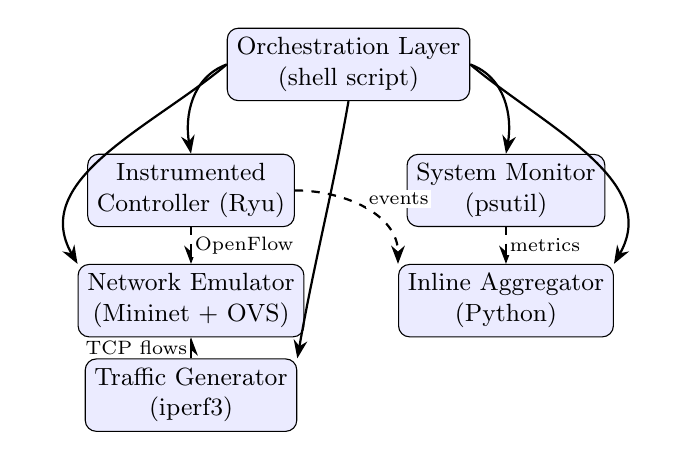
\begin{tikzpicture}[
  font=\small,
  box/.style={draw, rounded corners=4pt, minimum width=2.4cm,
              minimum height=0.65cm, align=center, fill=blue!8},
  arr/.style={-Stealth, thick},
  dasharr/.style={-Stealth, thick, dashed},
  lbl/.style={font=\scriptsize, fill=white, inner sep=1pt}
]
  % Left column
  \node[box] (ctrl)  at (0, 2.6)  {Instrumented\\Controller (Ryu)};
  \node[box] (mn)    at (0, 1.2)  {Network Emulator\\(Mininet + OVS)};
  \node[box] (traf)  at (0, 0)    {Traffic Generator\\(iperf3)};
  % Right column
  \node[box] (sys)   at (4.0, 2.6) {System Monitor\\(psutil)};
  \node[box] (agg)   at (4.0, 1.2) {Inline Aggregator\\(Python)};
  % Top centre
  \node[box] (orch)  at (2.0, 4.2) {Orchestration Layer\\(shell script)};

  % Orchestrator to left column (arrive at top edges)
  \draw[arr] (orch.west)  to[out=200, in=100] (ctrl.north);
  \draw[arr] (orch.west)  to[out=220, in=120] (mn.north west);
  \draw[arr] (orch.south) to[out=260, in=80]  (traf.north east);
  % Orchestrator to right column (arrive at top edges)
  \draw[arr] (orch.east)  to[out=340, in=80]  (sys.north);
  \draw[arr] (orch.east)  to[out=320, in=60]  (agg.north east);

  % Controller → Network Emulator (OpenFlow, left side vertical)
  \draw[dasharr] (ctrl.south) -- node[lbl, right]{OpenFlow} (mn.north);

  % Traffic Generator → Network Emulator (TCP flows, left side vertical)
  \draw[dasharr] (traf.north) -- node[lbl, left]{TCP flows} (mn.south);

  % System Monitor → Inline Aggregator (metrics, right side vertical)
  \draw[dasharr] (sys.south)  -- node[lbl, right]{metrics}   (agg.north);

  % Controller → Inline Aggregator (events, diagonal)
  \draw[dasharr] (ctrl.east)  to[out=0, in=90]
        node[lbl, above right, pos=0.5]{events} (agg.north west);

\end{tikzpicture}
\caption{Testbed architecture. The orchestration layer coordinates
all components; the aggregator consolidates per-run outputs.}
\label{fig:architecture}
\end{figure}

\subsection{Instrumented Controller}

The controller component is a custom Ryu~\cite{RyuFramework}
application that extends standard MAC-learning L2 switching
with three instrumentation layers. First, every Packet-In
event is timestamped on arrival using \texttt{time.perf\_counter()};
the processing time to FlowMod dispatch is recorded in
microsecond resolution to a per-run CSV file (\texttt{flow\_events.csv}).
This enables direct measurement of controller processing latency,
independent of network RTT. Reporting both the median (p50) and
95th-percentile (p95) of these per-event times is essential:
as Xiong et al.~\cite{Xiong2016QueueingSDN} and the IETF BMWG
note, mean latency does not reflect tail behavior in event-driven
systems under bursty load, and it is precisely the tail events
that reveal controller saturation and topology-driven anomalies.
Second, aggregate Packet-In and
FlowMod counts are written to a separate CSV
(\texttt{controller\_metrics.csv}) at one-second intervals via
a background greenthread (\texttt{hub.spawn}), ensuring the
logger does not block the main event loop. Third, the output
directory is injected via the \texttt{OUTDIR} environment
variable, allowing the orchestrator to direct each run's output
to an isolated directory without modifying controller code.

\subsection{Network Emulator and Topology Layer}

Mininet~\cite{Lantz2010Mininet} provides network emulation
using Open vSwitch~\cite{ovs} with TCLink. Topologies are
defined as Python classes inheriting from Mininet's \texttt{Topo}
base class. Currently, the testbed ships three built-in
topologies: star, fat-tree, and mesh. Adding a new topology
requires implementing a single \texttt{build(self, n)} method
and registering it with a one-line entry in the topology
factory. This design allows researchers to plug in any Mininet-
compatible topology without modifying the rest of the pipeline.

\subsection{Traffic Generator}

iperf3~\cite{iperf3} servers are started on each host at
unique port numbers (base port $+$ host index) and allowed
one second to bind before traffic begins. The traffic
generator maintains a precise inter-flow interval of
$1/\text{FPS}$ seconds using wall-clock timing with sleep
compensation to absorb scheduling jitter. For each flow,
source and destination hosts are selected uniformly at
random without replacement using a deterministic seed
that is unique per (topology, host count, flow rate,
repetition) tuple. Flows run concurrently as subprocesses,
creating overlapping TCP connections that generate simultaneous
Packet-In events and stress the controller in a way that
single-flow benchmarks may not.

\subsection{System Monitor}

A companion Python process uses \texttt{psutil}~\cite{psutil}
to record the controller process's CPU utilization, resident
memory (RSS), and thread count at one-second intervals for
the duration of each run. CPU percentage is primed with an
initial non-blocking call before sampling begins, following
psutil best practice. The monitor runs as a separate OS
process to avoid any GIL contention with the controller.

\subsection{Orchestration and Reproducibility}

The master shell script (\texttt{run\_experiment.sh}) accepts
topology, host count, flow rate, run duration, flow duration,
and seed as command-line arguments. Algorithm~\ref{alg:pipeline}
shows the full orchestration logic. Seeds are computed
deterministically as $\text{seed} = 1000 + N \cdot 10 +
\text{FPS} + \text{rep}$, guaranteeing that any individual
run can be exactly reproduced from its parameter tuple alone.
The matrix scripts iterate over all (topology, $N$, FPS,
repetition) combinations and invoke \texttt{run\_experiment.sh}
unattended for the full factorial sweep.

\begin{figure}[t]
\begin{algorithmic}[1]
\small
\REQUIRE topology $T$, host count $N$, flow rate $F$,
         duration $D$, seed $s$, output directory \textit{out}
\STATE Clean residual Mininet state (\texttt{mn -c})
\STATE Set \texttt{OUTDIR} $\leftarrow$ \textit{out}
\STATE Launch Ryu controller $\rightarrow$ background PID $p_c$
\STATE Launch system monitor (psutil, PID $p_c$) $\rightarrow$ background
\STATE \textbf{sleep}(1)\hfill\COMMENT{Allow controller to bind}
\STATE Launch Mininet($T$, $N$) + iperf3 traffic gen (seed $s$, FPS $F$, dur $D$)
\STATE \textbf{wait} for all iperf3 clients to complete
\STATE Kill system monitor; kill Ryu controller
\STATE \textbf{sleep}(1)\hfill\COMMENT{Allow file handles to flush}
\STATE Run \texttt{aggregate\_results.py} $\rightarrow$ append row to \texttt{summary.csv}
\IF{aggregation succeeded}
  \STATE Delete \texttt{iperf\_json/}, \texttt{ryu\_stdout.log},
         \texttt{mininet\_iperf.log}
  \STATE Retain \texttt{flow\_events.csv}, \texttt{controller\_metrics.csv},
         \texttt{system\_metrics.csv}, \texttt{traffic\_meta.json}
\ELSE
  \STATE Retain all raw files for manual inspection
\ENDIF
\end{algorithmic}
\caption{Testbed orchestration pipeline (\texttt{run\_experiment.sh}).}
\label{alg:pipeline}
\end{figure}

\subsection{Metrics and Aggregation}

After each run, the inline aggregator (\texttt{aggregate\_results.py})
reads the three output CSVs and the metadata JSON, computes
the following metrics, and appends one row to a master
summary CSV:

\begin{itemize}
  \item \textbf{Throughput (Gbps):} sum of \texttt{bits\_per\_second}
  across all iperf3 flows, converted from the per-flow JSON output.
  \item \textbf{Packet-In rate (pkts/sec):} mean of the
  per-second counts in \texttt{controller\_metrics.csv}.
  \item \textbf{Processing latency p50 and p95 (ms):} 50th and
  95th percentiles of \texttt{proc\_time\_ms} across all events
  in \texttt{flow\_events.csv}.
  \item \textbf{CPU utilization (\%):} mean CPU percent across
  all one-second samples in \texttt{system\_metrics.csv}.
  \item \textbf{Memory (MB):} mean RSS across all samples.
\end{itemize}

% ── IV. Testbed Validation ────────────────────────────────────
\section{Testbed Validation: A Case Study with Ryu}
\label{sec:demo}

\subsection{Experimental Configuration}

To validate the testbed and demonstrate its measurement
capabilities, we run a full factorial experiment using the
Ryu~\cite{RyuFramework} controller (v4.34, OpenFlow~1.3)
across two topologies, five host counts, and four flow rates.
Table~\ref{tab:params} summarizes the configuration.
All experiments run on a single VirtualBox VM (Ubuntu~24.04,
16~vCPUs, 16~GB RAM). The full 400-run sweep was executed
unattended using the matrix scripts.

\begin{table}[t]
\centering
\caption{Validation Experiment Parameters}
\label{tab:params}
\renewcommand{\arraystretch}{1.1}
\begin{tabular}{ll}
\toprule
\textbf{Parameter} & \textbf{Values} \\
\midrule
Topologies        & Star, Fat-Tree \\
Host count ($N$)  & 4, 8, 16, 32, 64 \\
Flow rate (FPS)   & 25, 50, 100, 200 flows/sec \\
Flow duration     & 2 seconds \\
Run duration      & 20 seconds \\
Repetitions       & 10 (distinct seeds per config) \\
Total runs        & 400 (200 per topology) \\
Controller        & Ryu v4.34 (OpenFlow~1.3) \\
Emulator          & Mininet + OVSSwitch + TCLink \\
Traffic tool      & iperf3 (TCP, JSON output) \\
\bottomrule
\end{tabular}
\end{table}

\subsection{Throughput and Packet-In Rate}

Fig.~\ref{fig:throughput_packetin} shows aggregate throughput
and Packet-In rate versus flow rate. Fat-tree achieves higher
throughput at most configurations (2938 vs.\ 2491\,Gbps at
200\,fps), demonstrating that the testbed correctly captures
topology-driven throughput differences. The fat-tree topology
generates substantially more Packet-In events because each
aggregation switch contributes independently to the controller
event stream, producing up to $5\times$ more events than the
star topology at the same flow rate. Both topologies show a
slight Packet-In decline at 200\,fps as flow table entries are
reused---a behavioral nuance that only per-event instrumentation
can reveal.

\begin{figure}[t]
\centering
  \subfigure[Aggregate throughput vs.\ flow rate]{%
    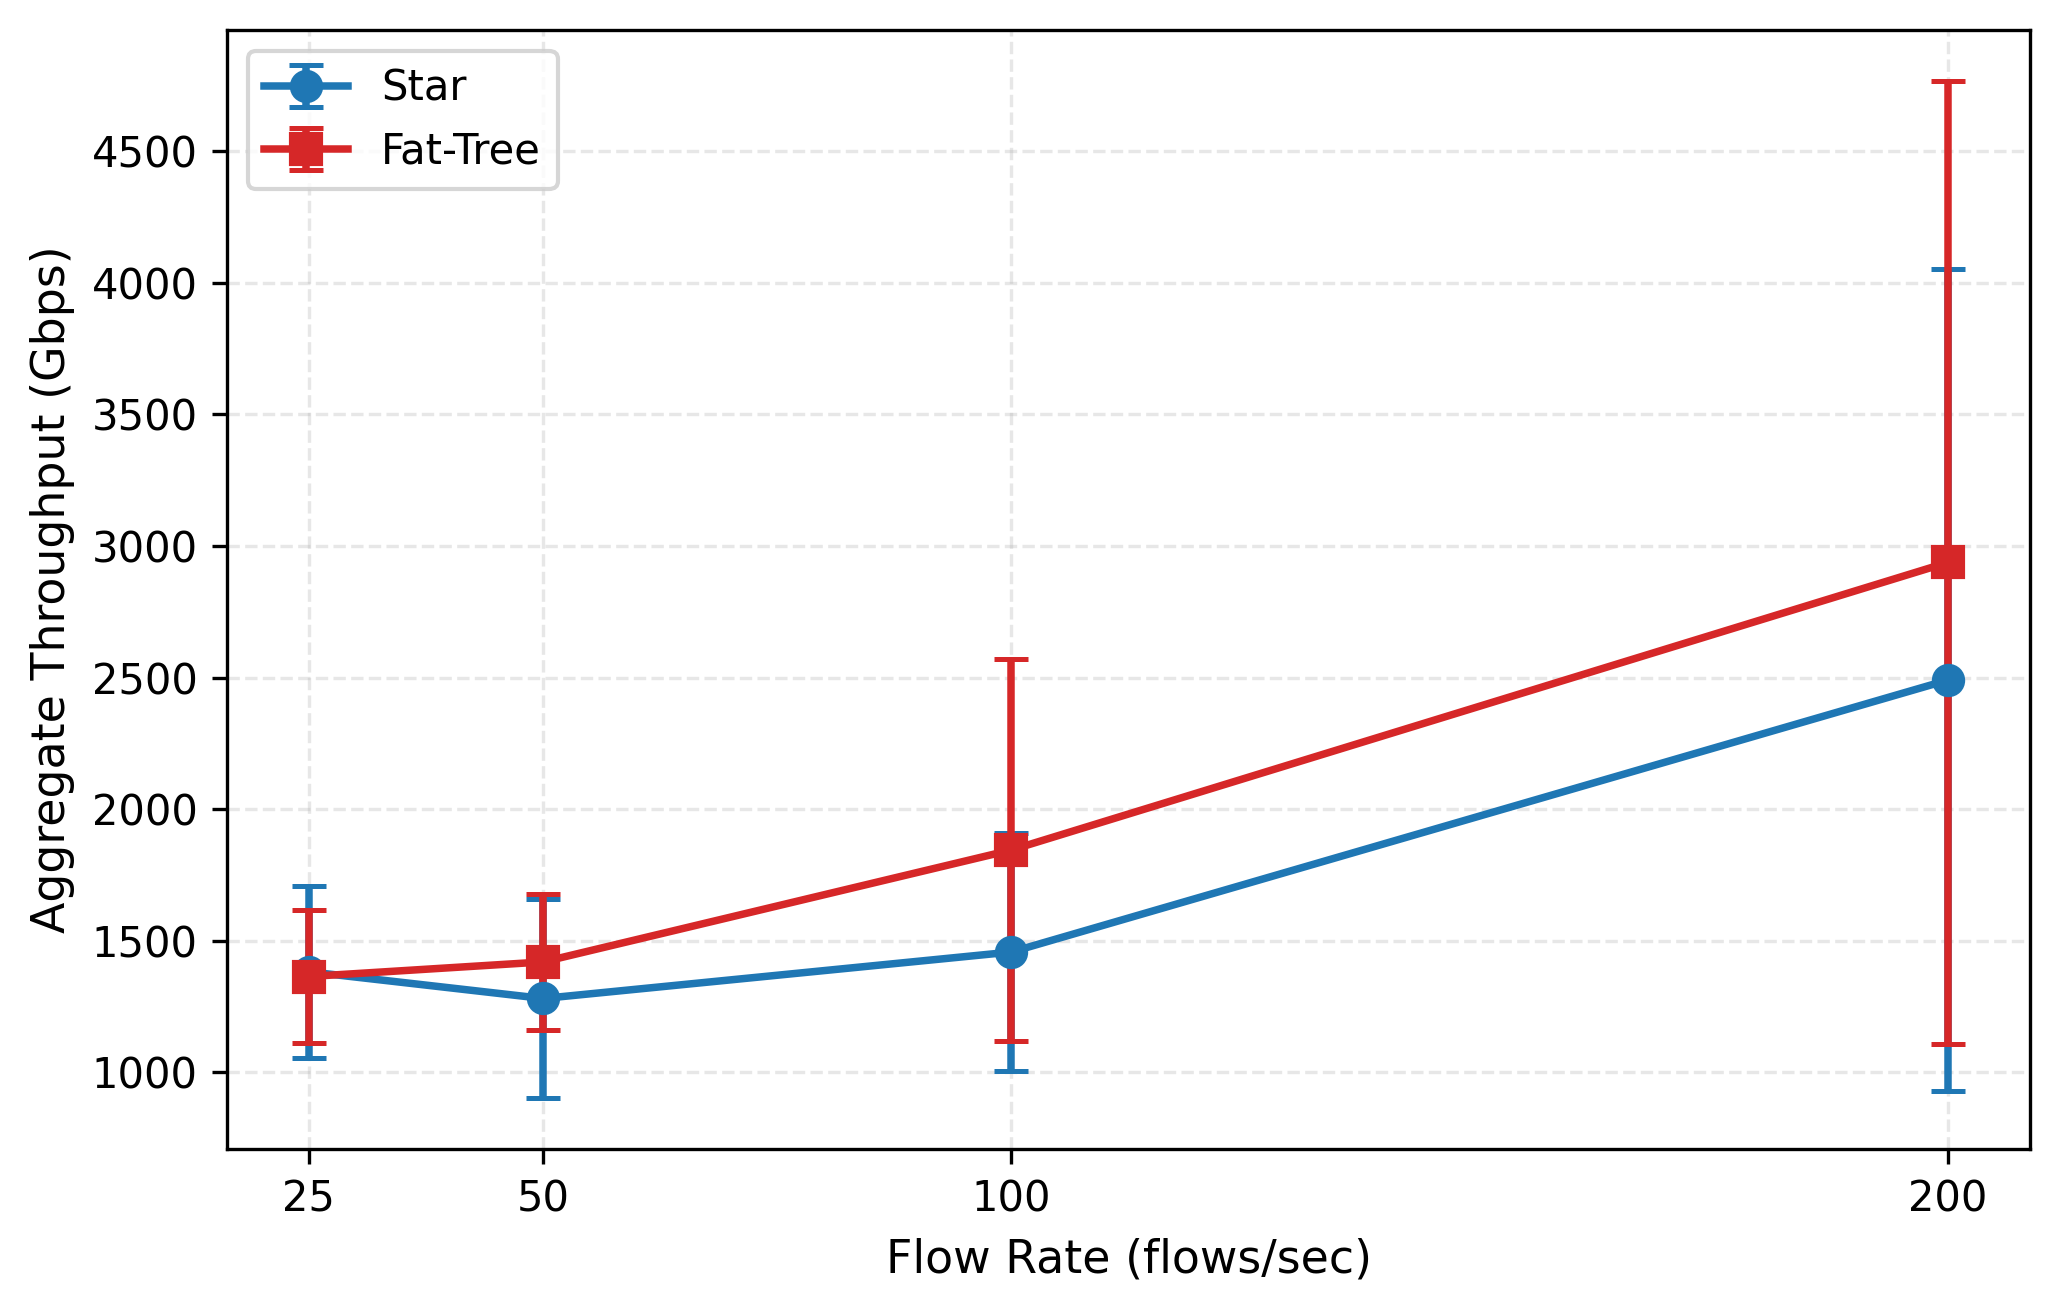
\includegraphics[width=0.48\linewidth]{figures/fig1_throughput_vs_fps}
  }
  \hfill
  \subfigure[Packet-In rate vs.\ flow rate]{%
    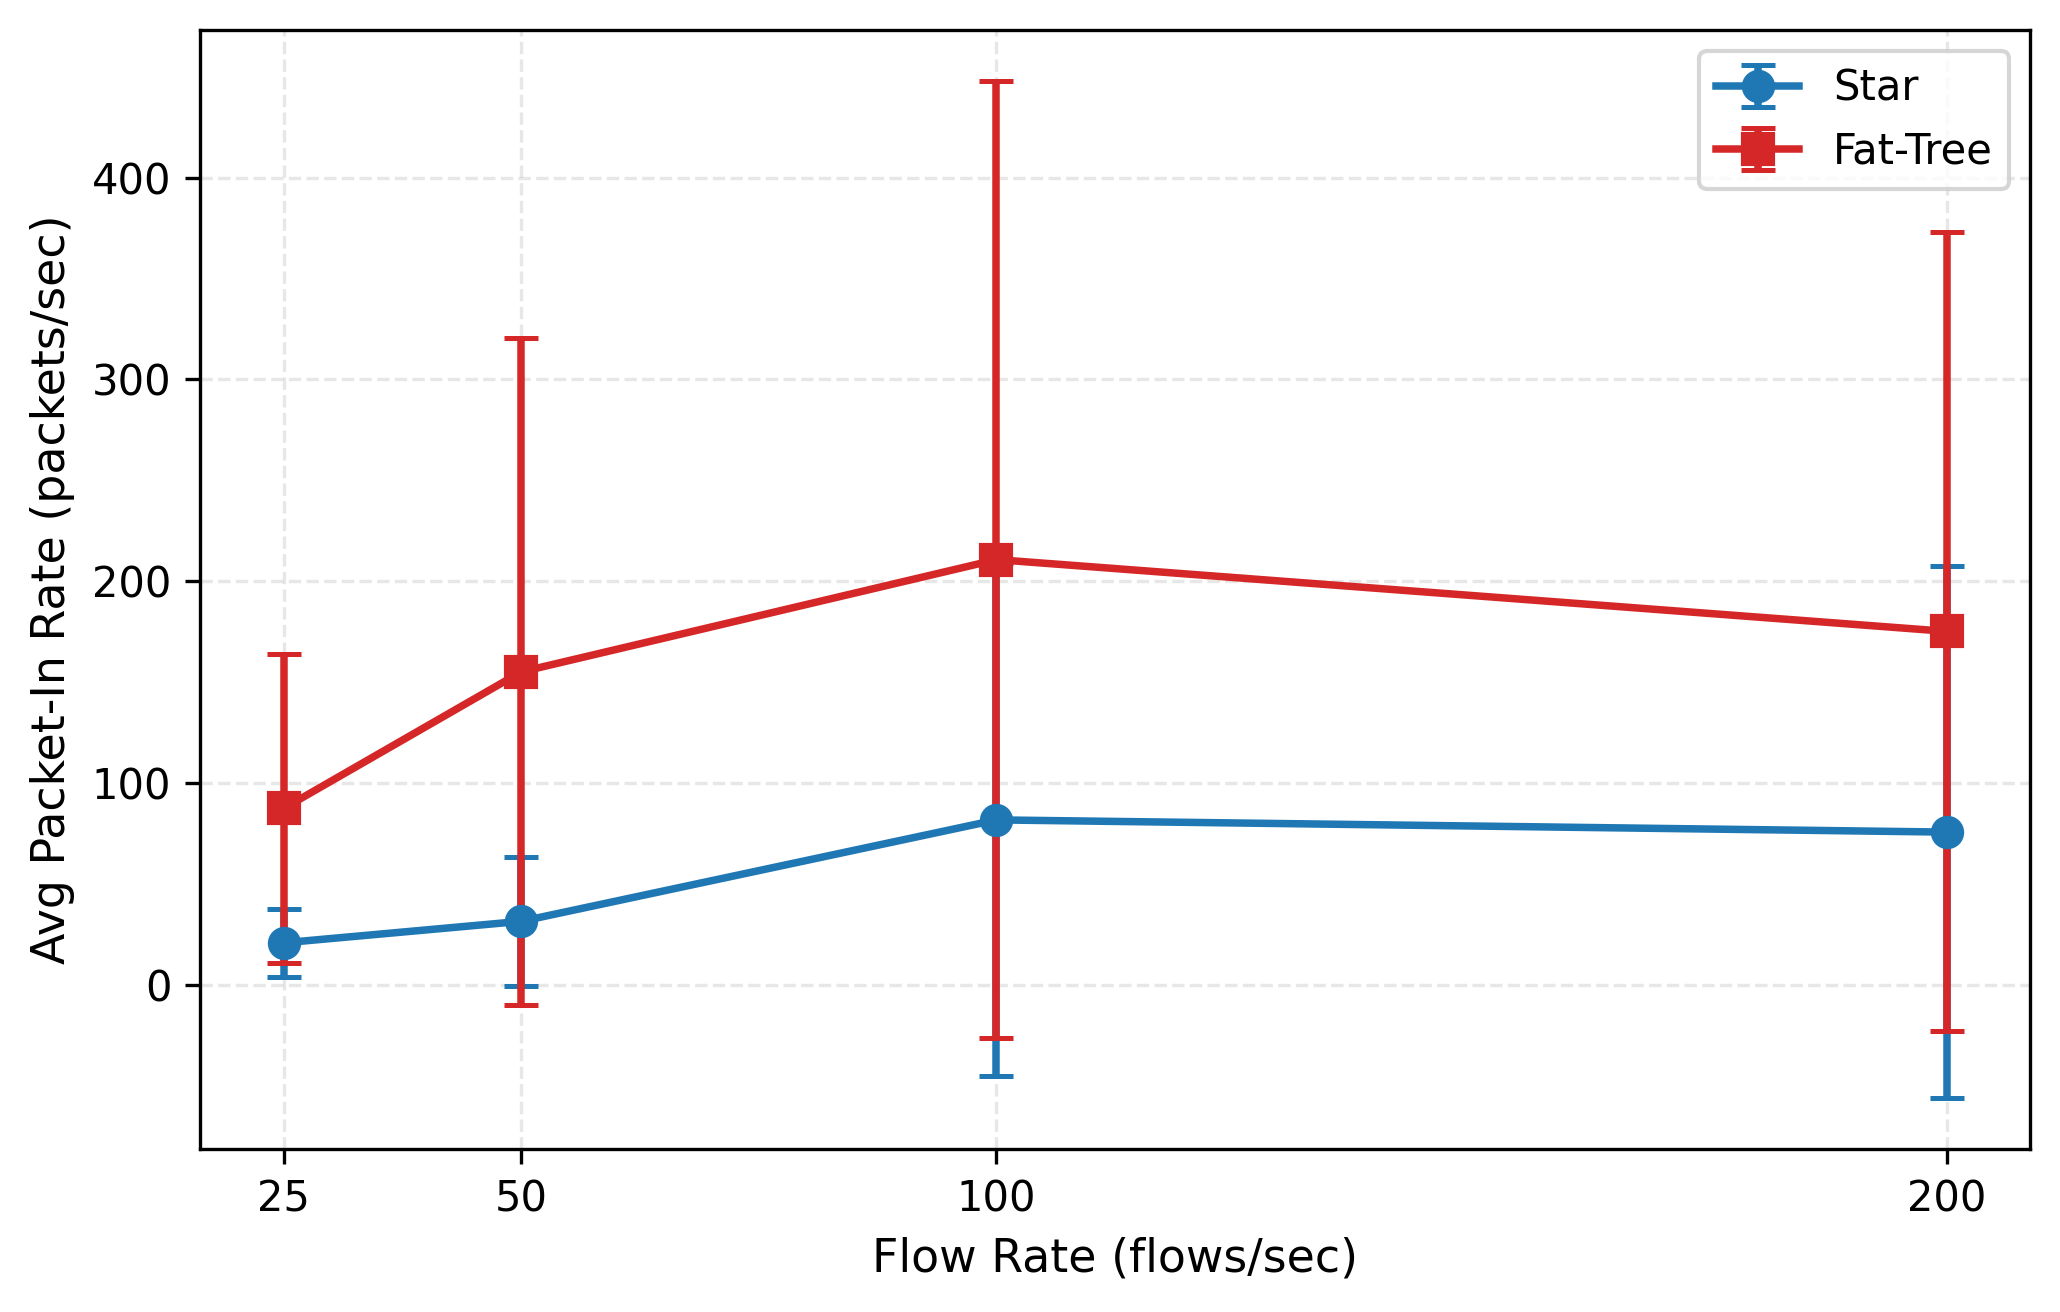
\includegraphics[width=0.48\linewidth]{figures/fig2_packetin_vs_fps}
  }
\caption{Throughput and Packet-In rate vs.\ flow rate.
Error bars show one standard deviation across 10 repetitions.}
\label{fig:throughput_packetin}
\end{figure}

\subsection{Per-Event Processing Latency}

Fig.~\ref{fig:latency} presents the most significant
demonstration of testbed capability: per-event processing
latency at p50 and p95 across topologies and flow rates.
The p50 latency is near zero for both topologies, confirming
that median-latency measurements---the only metric available
in prior work---would show no meaningful difference between
topologies. However, the p95 latency tells a strikingly
different story: star topology p95 peaks at 10.44\,ms at
50\,fps before declining, while fat-tree p95 grows gradually
from 3.04\,ms to 6.80\,ms, consistent with queuing theory
predictions~\cite{Xiong2016QueueingSDN}.

This p50/p95 divergence is directly attributable to the
testbed's per-event instrumentation. No existing open-source
benchmarking tool measures Packet-In-to-FlowMod latency at
event granularity; prior studies using ping and iPerf RTT
report only end-to-end delay, which conflates network latency
with controller processing latency.

\begin{figure}[t]
\centering
  \subfigure[Processing latency (p50 and p95) vs.\ flow rate]{%
    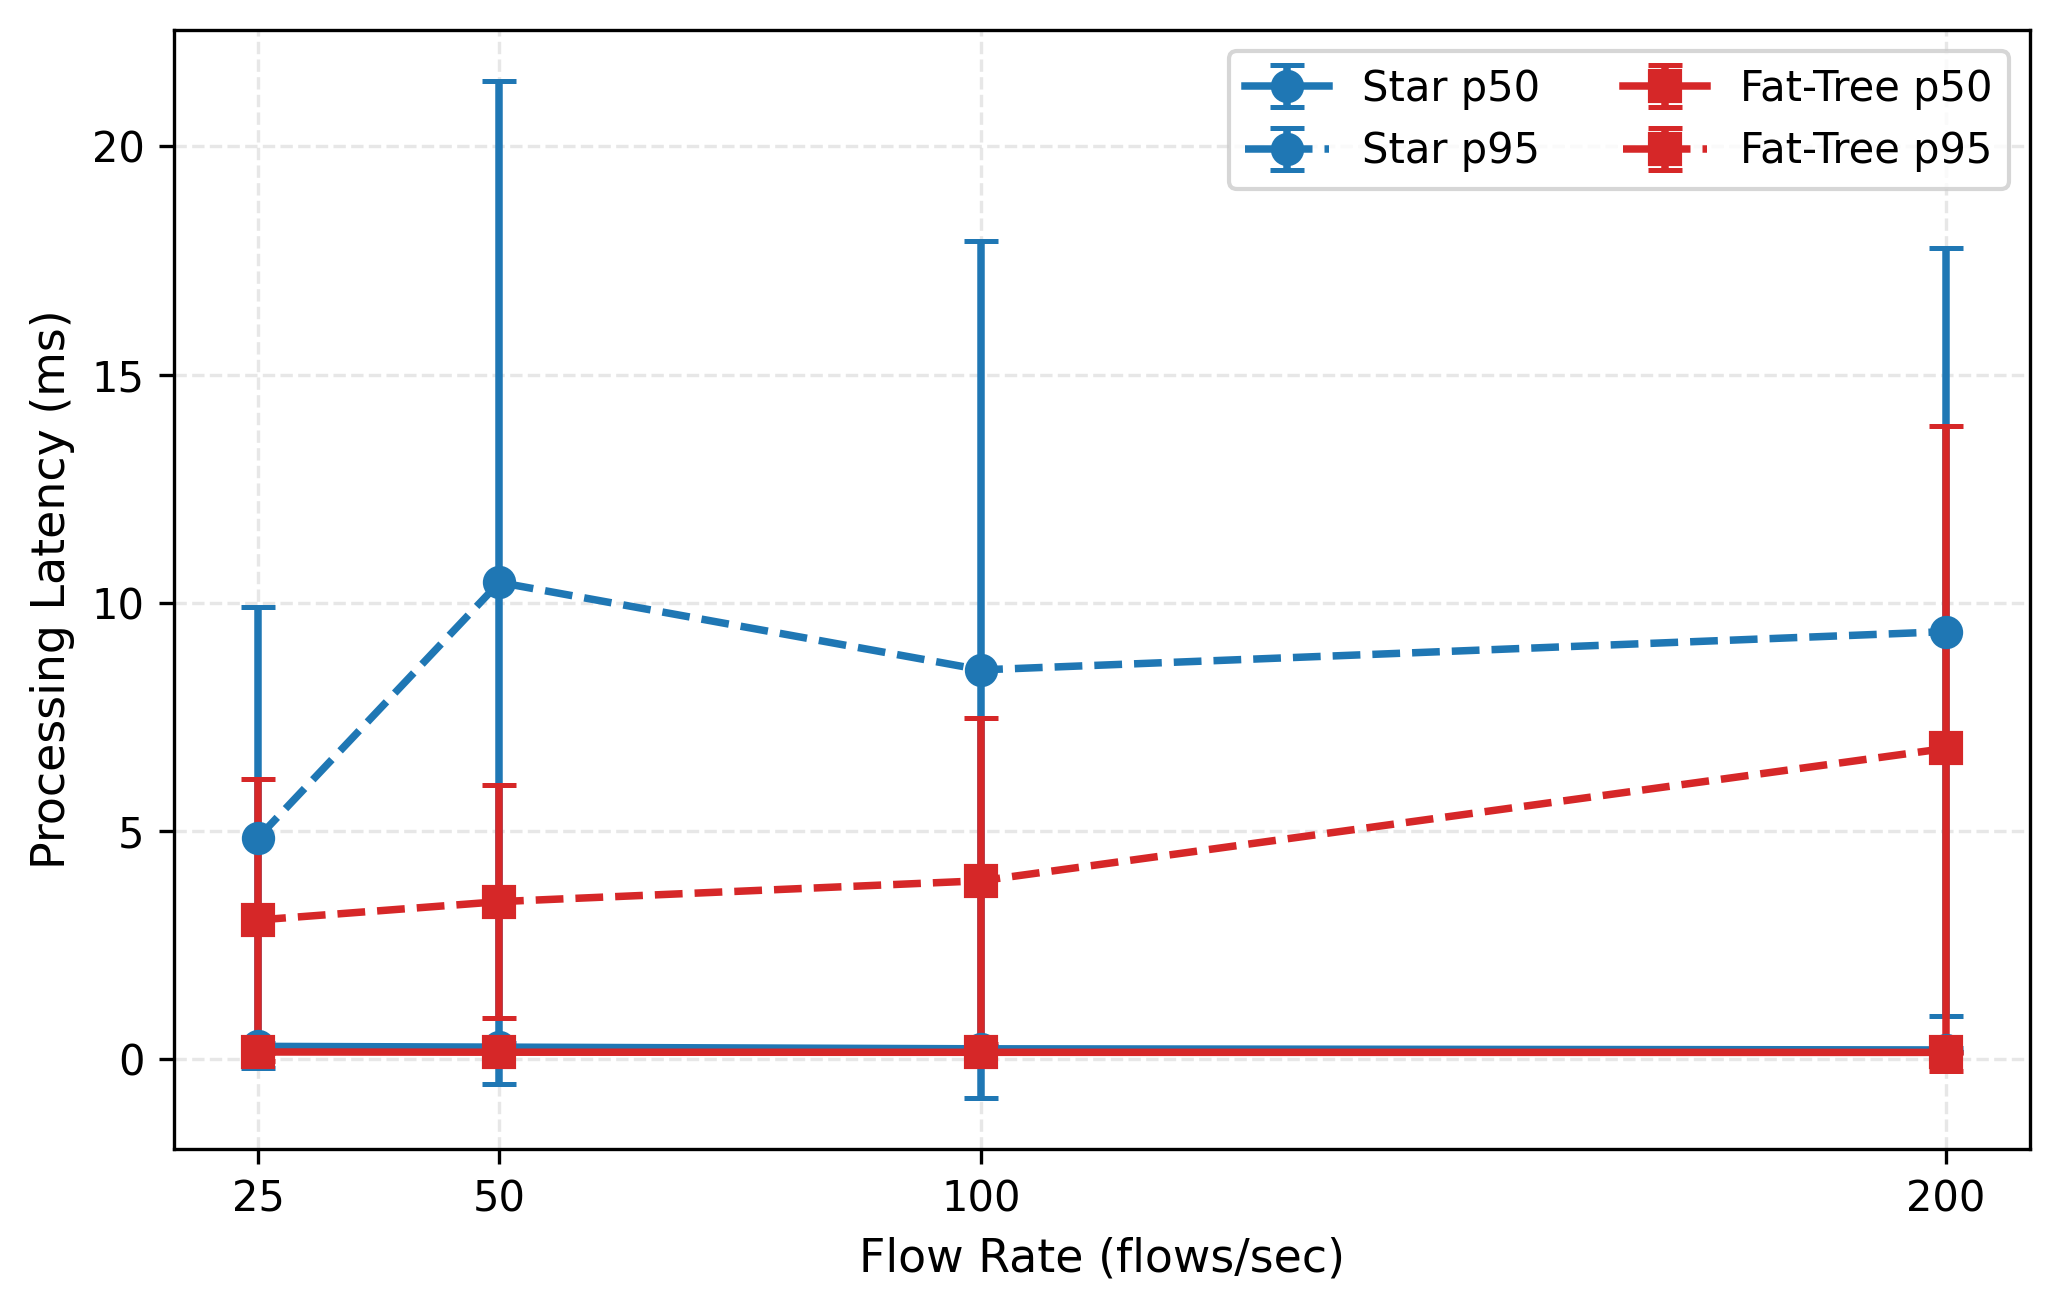
\includegraphics[width=0.48\linewidth]{figures/fig3_latency_vs_fps}
  }
  \hfill
  \subfigure[CPU usage vs.\ flow rate]{%
    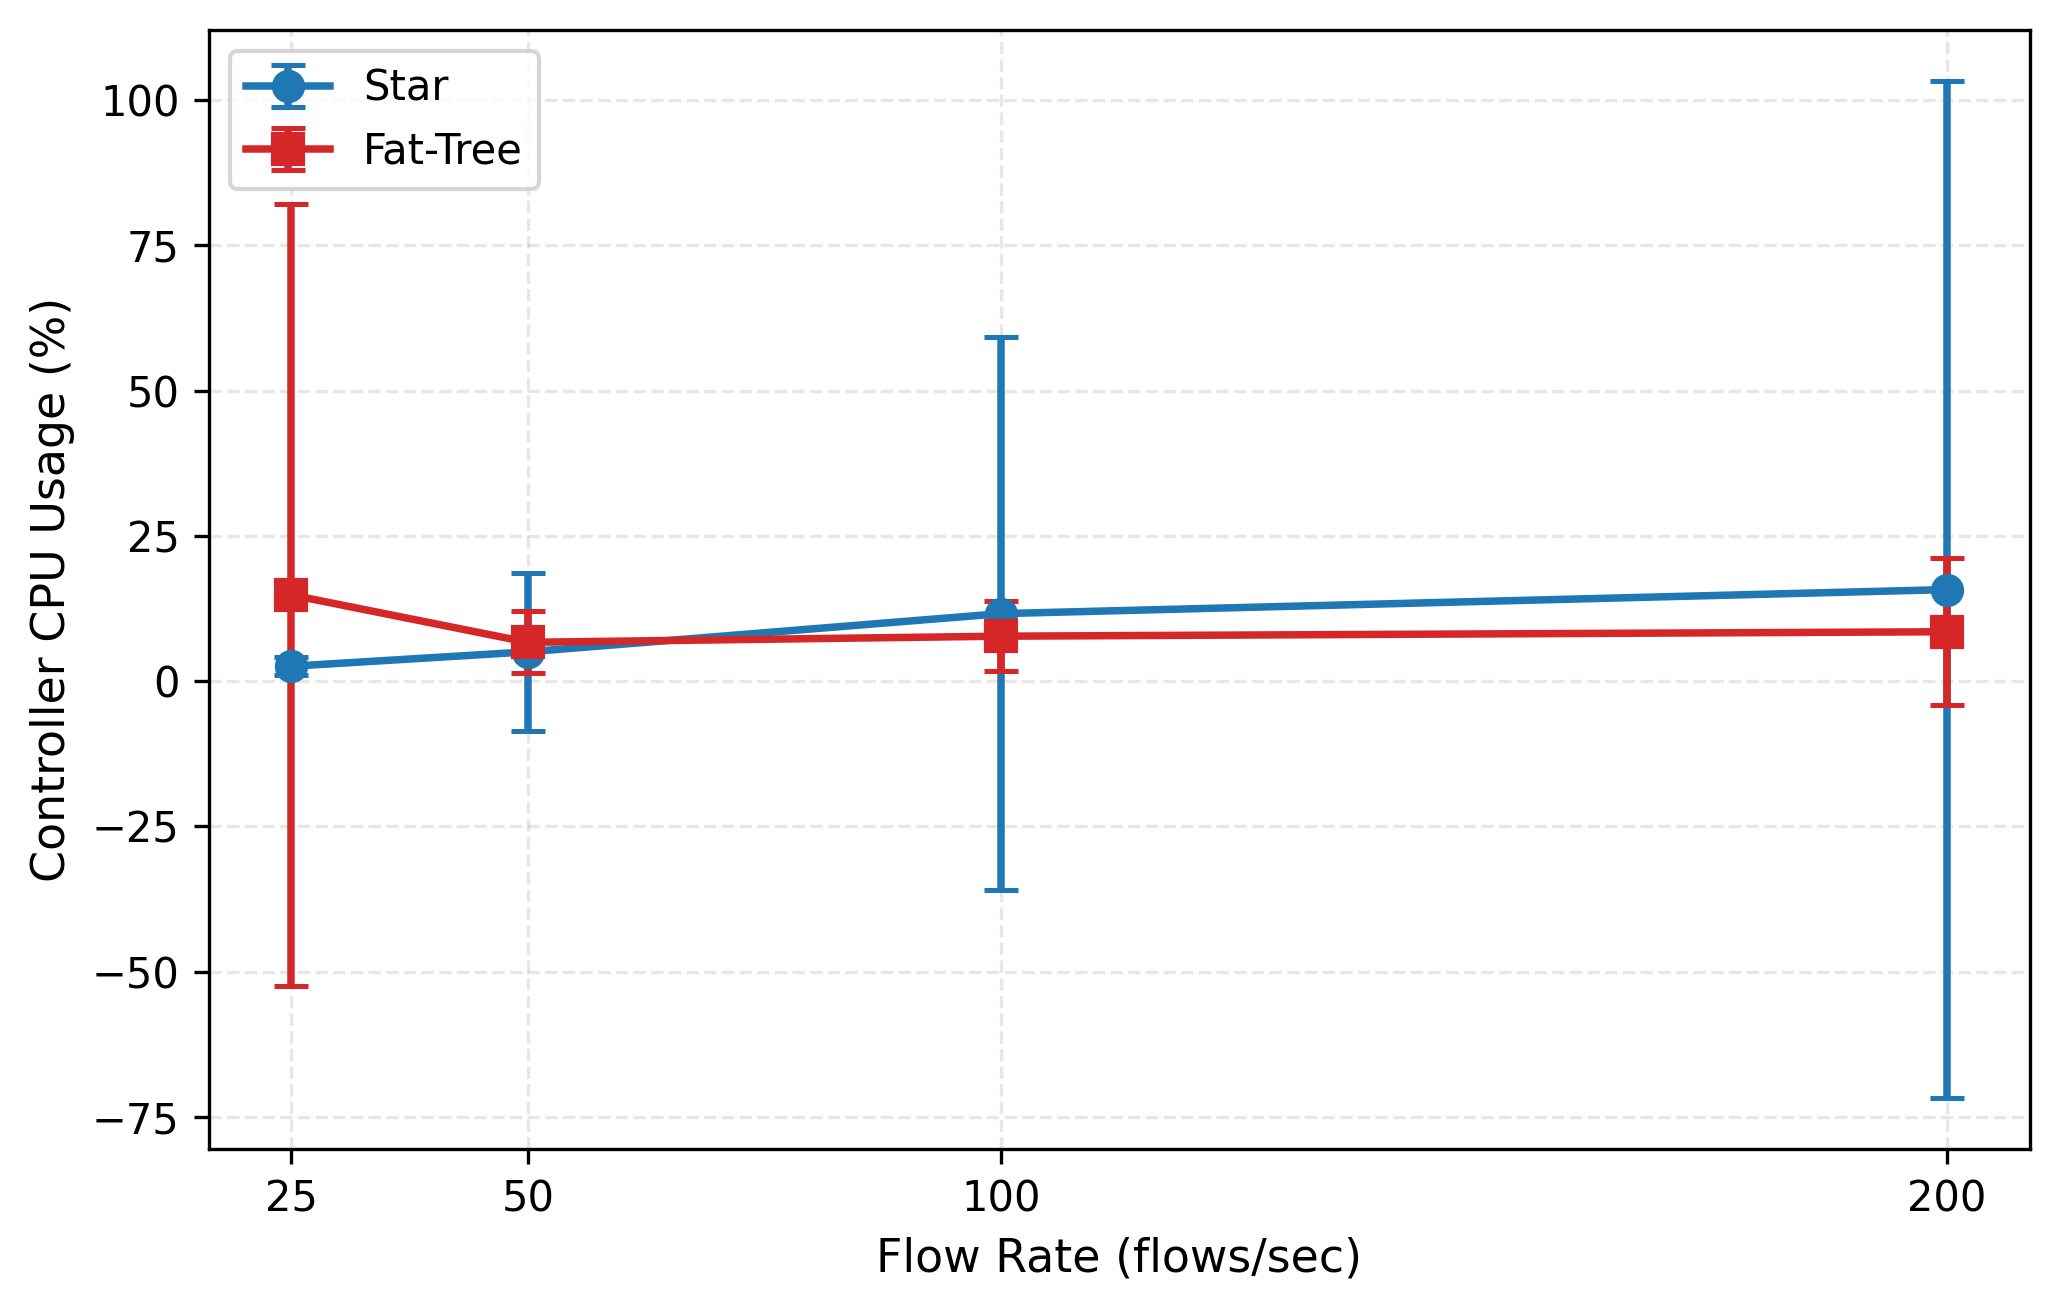
\includegraphics[width=0.48\linewidth]{figures/fig4_cpu_vs_fps}
  }
\caption{Processing latency and CPU usage vs.\ flow rate.
p50 is near zero for both topologies; p95 reveals large
topology-dependent differences invisible to RTT-based
measurements. Error bars show one standard deviation.}
\label{fig:latency}
\end{figure}

\subsection{Scalability with Host Count}

Fig.~\ref{fig:scalability} and Table~\ref{tab:hosts}
reveal a critical scalability divergence as host count increases.
Star topology p95 latency grows 24.4$\times$ from 0.73\,ms
at $N{=}4$ to 17.81\,ms at $N{=}64$, whereas fat-tree p95
grows only 10.9$\times$ (0.68 to 7.44\,ms), remaining
2.4$\times$ lower at maximum scale. The star's p95 plateaus
near 17\,ms between $N{=}32$ and $N{=}64$, suggesting
saturation of a burst-driven phenomenon.

\begin{figure}[t]
\centering
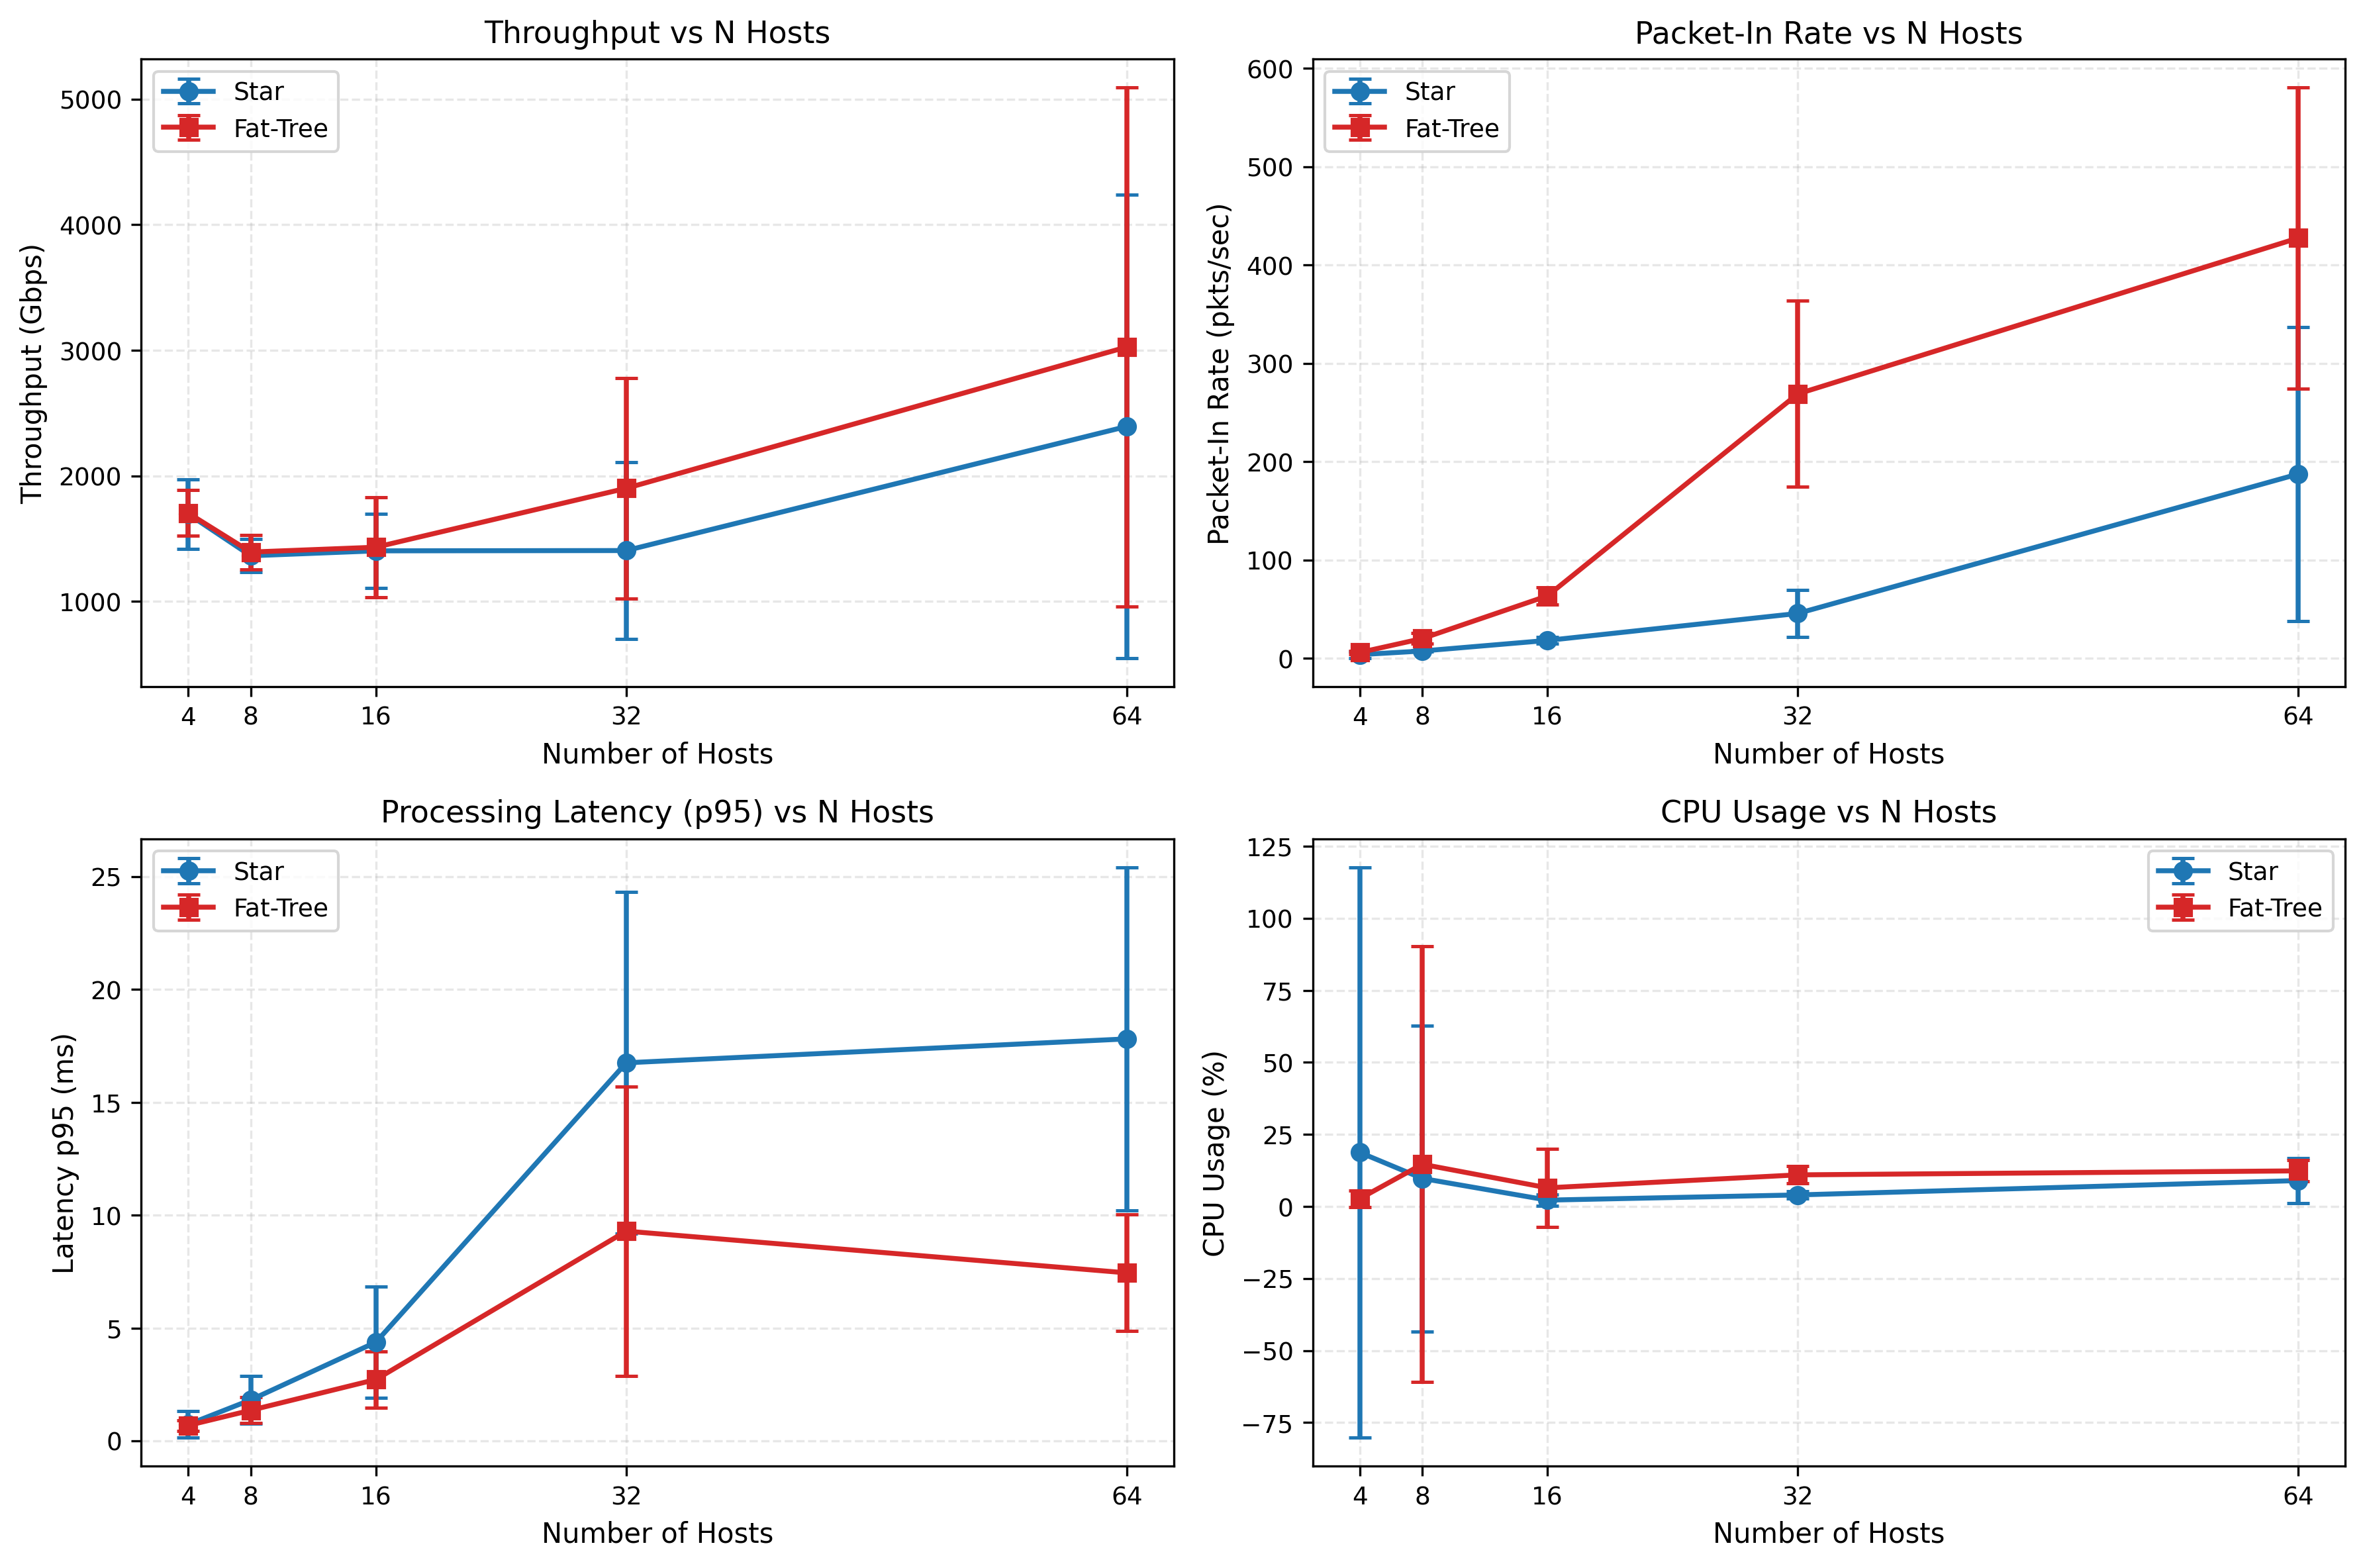
\includegraphics[width=\columnwidth]{figures/fig3_scalability_vs_hosts}
\caption{Scalability: throughput, Packet-In rate, p95 latency,
and CPU vs.\ host count. Star p95 plateaus at ${\sim}17$\,ms
beyond $N{=}32$; fat-tree remains lower across all scales.}
\label{fig:scalability}
\end{figure}

\begin{table}[t]
\centering
\caption{Mean Performance Metrics by Topology and Host Count}
\label{tab:hosts}
\renewcommand{\arraystretch}{1.1}
\begin{tabular}{llrrrr}
\toprule
\textbf{Topo.} & $N$ &
\makecell{\textbf{Tput}\\\textbf{(Gbps)}} &
\makecell{\textbf{Pkt-In}\\\textbf{(pkt/s)}} &
\makecell{\textbf{p95 Lat}\\\textbf{(ms)}} &
\makecell{\textbf{CPU}\\\textbf{(\%)}} \\
\midrule
Fat-Tree & 4  & 1703.93 & 5.88   & 0.68  & 2.70  \\
Fat-Tree & 8  & 1393.19 & 20.03  & 1.35  & 14.66 \\
Fat-Tree & 16 & 1431.88 & 63.42  & 2.72  & 6.47  \\
Fat-Tree & 32 & 1901.14 & 268.79 & 9.29  & 10.98 \\
Fat-Tree & 64 & 3026.39 & 427.36 & 7.44  & 12.36 \\
\midrule
Star     & 4  & 1696.51 & 3.69   & 0.73  & 18.78 \\
Star     & 8  & 1363.72 & 7.40   & 1.82  & 9.74  \\
Star     & 16 & 1402.91 & 18.16  & 4.37  & 2.21  \\
Star     & 32 & 1405.18 & 45.58  & 16.75 & 4.01  \\
Star     & 64 & 2393.71 & 187.36 & 17.81 & 8.99  \\
\bottomrule
\end{tabular}
\end{table}

% ── V. Discussion ─────────────────────────────────────────────
\section{Discussion}
\label{sec:discussion}

\subsection{What the Testbed Revealed}

The validation experiments surface five findings that
demonstrate the testbed's measurement capabilities.
\textbf{(F1)} Topology and host count drive p95 latency
far more than flow rate in the tested range---a finding
only accessible through systematic multi-dimensional
parameter sweeps, a capability that prior open-source tools have not yet offered.
\textbf{(F2)} The p50/p95 latency gap demonstrates that
tail behavior is driven by a small fraction of events and
is invisible to median-based or RTT-based measurements.
\textbf{(F3)} Star topology p95 latency grows
near-quadratically with host count (0.73~$\to$~17.81\,ms,
24.4$\times$) but saturates between $N{=}32$ and $N{=}64$,
consistent with a MAC learning burst of $N(N-1)/2$ unique
host pairs temporarily saturating the controller's event queue.
\textbf{(F4)} Fat-tree topology partitions MAC learning
across aggregation switches, bounding burst intensity to
${\leq}6$ host pairs per switch regardless of total
network size, which explains its 2.4$\times$ lower tail
latency at scale. \textbf{(F5)} CPU utilization remains
below 16\% for both topologies, confirming that the
observed latency anomalies are event-queue driven rather
than compute-resource limited.

Critically, the MAC burst phenomenon in~(F3) and~(F4) was
discovered only because the testbed instruments individual
Packet-In events: a study using only aggregate RTT
measurements would observe a higher average latency for
star topologies but could not distinguish burst-phase
from steady-state behavior, nor identify the $N(N-1)/2$
scaling relationship.

\subsection{Limitations of the Demonstration}

The current demonstration uses a single-threaded controller
(Ryu). Ryu's Python Global Interpreter Lock (GIL) prevents
true parallel event processing~\cite{Shalimov2013HCprobe},
making it a tractable but architecturally constrained
baseline. The testbed is designed for straightforward
extension to multi-threaded or distributed controllers
such as ONOS~\cite{Berde2014ONOS} or OpenDaylight.

Emulation fidelity is a secondary limitation: Mininet
with OVSSwitch in VirtualBox introduces timing noise not
present in physical hardware deployments. Absolute
throughput values reflect the emulated environment;
relative comparisons across topologies and configurations
remain valid.

\subsection{Testbed Roadmap}

The current release is a foundation; our planned development
focuses on upgrading the testbed itself along three stages.
\textbf{Containerization:} The most immediate priority is
replacing Mininet's network namespaces with per-host Docker
containers, giving each emulated node a fully isolated
filesystem, process space, and network stack. Running the
controller, hosts, and traffic generator as containers
makes the topology behave closer to a real deployment and
makes the entire testbed portable---any researcher could
bring it up with a single \texttt{docker compose up} command
on any machine, with no manual dependency installation.
\textbf{Configurable infrastructure:} Building on the
containerized foundation, we plan to expose link-level
parameters---bandwidth, latency, and loss rate---as
first-class configuration alongside topology and traffic
parameters, enabling researchers to model a wider range
of network conditions without modifying any code.
\textbf{Web-based interface:} The longer-term goal is a
browser-based frontend through which a researcher can
select a topology, set all experiment parameters, launch
a run, and retrieve result plots---removing the command-line
requirement entirely and making the testbed accessible to
the broader SDN research community.

% ── VI. Conclusion ─────────────────────────────────────────
\section{Conclusion}
\label{sec:conclusion}

We presented an open-source, plug-and-play SDN controller
benchmarking testbed that addresses three core limitations
of the current landscape: the reliance on synthetic traffic
in established tools such as CBench and OFLOPS, the
lack of statistical rigor and automation in academic
emulation studies, and the absence of any open-source
implementation of the IETF's RFC~8456 benchmarking
methodology.

The testbed contributes a seed-controlled automated pipeline,
per-event controller instrumentation that separates p50
from p95 processing latency, concurrent realistic TCP
traffic via iperf3, and a plug-and-play topology and
parameter system. A 400-run validation study using Ryu
across star and fat-tree topologies confirms that the
testbed successfully captures statistically validated,
topology-dependent controller behavior---including a
MAC learning burst anomaly that is undetectable by
prior benchmarking approaches.

The testbed is publicly available at
\url{https://github.com/PLACEHOLDER/sdn-testbed}.
Planned development will progressively upgrade the tool
itself---toward containerized per-host isolation, richer
link-level configuration, and a web-based interface---with
the goal of making rigorous SDN controller benchmarking
accessible to the broader research community.

% ── References ─────────────────────────────────────────────
\bibliographystyle{IEEEtran}
\bibliography{references_icc2027}

\end{document}